\documentclass{article}

\usepackage[brazil]{babel}
\usepackage[utf8]{inputenc}
\usepackage{amsmath}
\usepackage{amsfonts}

\usepackage[section]{placeins}

\usepackage{graphicx}

\usepackage{color} %red, green, blue, yellow, cyan, magenta, black, white
\definecolor{mygreen}{RGB}{28,172,0} % color values Red, Green, Blue
\definecolor{mylilas}{RGB}{170,55,241}

\begin{document}

\begin{flushleft}
\textbf{FUNDAÇÃO GETÚLIO VARGAS} \\

\textbf{Escola de Pós-Graduação em Economia}

\textbf{Teoria Macroeconômica III - Lista 03}

Professor: Ricardo de Oliveira Cavalcanti

Monitora: Kátia Aiko Nishiyama Alves

Alunos: Samuel Barbosa e Gustavo Bulhões
\end{flushleft}

\section*{Exercício 01}
Neste exercício consideramos a economia de trocas estudada por Huggett (1993).

\subsection*{Item (a)}
Utilizando o limite de endividamento $\underline{a} = -2$ e seguindo os demais parâmetros em
Hugget (1993), obtemos as seguintes funções valor e política nos estados $e_H$ e $e_L$:

\begin{figure}[!h]
  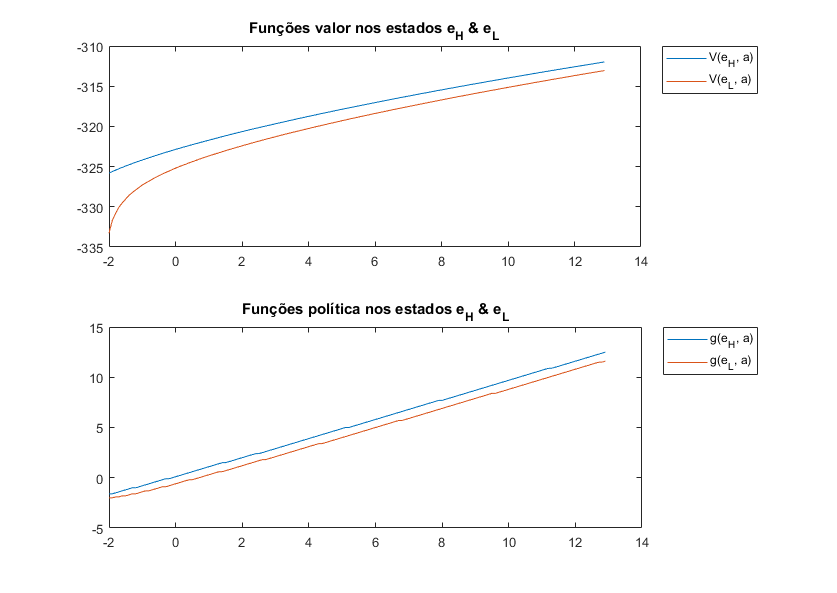
\includegraphics[scale=0.6]{ex1/ex1_1.png}
\end{figure}

\subsection*{Item (b)}

Código anexo.

\subsection*{Item (c)}

Observe que $$(M' - 1I) \lambda = 0 \iff M' \lambda = \lambda,$$ isto é, 
o autovetor associado ao autovalor unitário de $M'$ é uma 
distribuição invariante de $M'$. Ao normalizar este autovetor,
podemos interpretá-lo, no modelo de Huggett, como a probabilidade (ou proporção) 
estacionária de indivíduos em cada estado $(a, e)$.

\subsection*{Item (d)}

Podemos calcular a distribução invariante de M iterando $\lambda_{j+1} = \lambda_j M$ até
obter $\lambda_{j+1} = \lambda{j}$. Como esperado, a distribuição obtida é idêntica à
calculada no item anterior.

\subsection*{Item (e)}

Ainda com $\underline{a} = -2$ e definindo o preço inicial do ativo 
em $q = 1$, obtemos, inicialmente, excesso de oferta de 
crédito $z = 0.8796$.

\subsection*{Item (f)}

Ajustando iterativamente os preços, obtemos equilíbrio com $q = 1.0064$ quando $\underline{a} = -2$.

\subsection*{Item (g)}

A tabela a seguir apresenta os preços de equilíbrio nos estados $e_H$ e $e_L$,
para diferentes valores de $\underline{a}$. \\

\begin{center}
\begin{tabular}{cc}
	\hline $\underline{a}$ & $q$ \\ \hline
	-2  &  1.0064 \\
	-4  &  0.9968 \\
	-6  &  0.9949 \\
	-8  &  0.9939 \\
   -10  &  0.9933 \\
   -12  &  0.9931 \\ \hline
\end{tabular}
\end{center}

\end{document}

